% Evidence: frontend/src/theme/theme.ts; components/BottomNavigation.tsx;
% screens/AuthenticatedScreen.web.tsx:WebWorkspace; components/HandwritingLookup.tsx;
% components/ReadingQuiz.tsx; hooks/useWritingDocuments.ts; existing MVP screenshots.
Nhóm thiết kế giao diện NihonGO xoay quanh ba thao tác chính: tìm nội dung, thực hành và xem lại kết quả. Các màn hình duy trì điều hướng nhất quán, đồng thời điều chỉnh bố cục cho web và di động. Các hình dưới đây minh họa những thành phần giao diện với dữ liệu mẫu.

% Keep each component crop next to its description; avoid floating to MVP pages.
\newcommand{\uicomponentfigure}[3]{%
  \par\smallskip\noindent\begin{minipage}{\linewidth}
    \centering #1
    \captionof{figure}{#2}\label{#3}
  \end{minipage}\par\medskip}

\Needspace{8cm}
\noindent\textbf{Phong cách giao diện.}
Màu cam làm nổi bật hành động chính và mục đang chọn trên nền sáng. Thẻ nội dung bo góc, chữ có phân cấp và biểu tượng đi kèm nhãn. Hình~\ref{fig:ui-content-card} minh họa thẻ ôn tập với hướng dẫn, linh vật Momo và nút hành động chính.
\uicomponentfigure{
  
\includegraphics[width=8.4cm]{figures/ui-components/home-review-card.png}
}{Thẻ nội dung, phân cấp chữ và nút hành động chính}{fig:ui-content-card}

\Needspace{8cm}
\noindent\textbf{Tổ chức thông tin và điều hướng.}
Năm mục chính gồm Trang chủ, Luyện tập, Tra cứu, Bài học và Cá nhân. Thanh điều hướng nằm bên trái trên web rộng và ở phía dưới trên di động, màn hình hẹp. Mục đang mở được đánh dấu bằng màu và chỉ báo vị trí (Hình~\ref{fig:ui-navigation}).
\uicomponentfigure{
  \begin{minipage}[c]{3.3cm}
    \centering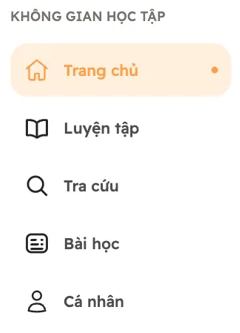
\includegraphics[height=4.1cm]{figures/ui-components/desktop-navigation.png}
  \end{minipage}\hspace{.5cm}
  \begin{minipage}[c]{10.5cm}
    \centering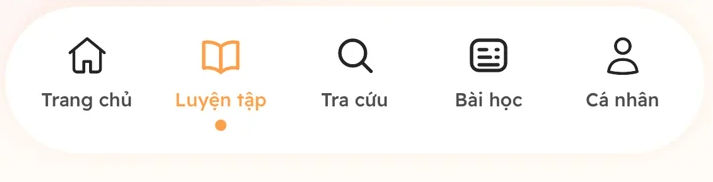
\includegraphics[width=10.5cm]{figures/ui-components/mobile-navigation.png}
  \end{minipage}
}{Thanh điều hướng bên trái trên web và thanh dưới trên di động}{fig:ui-navigation}

\Needspace{7cm}
\noindent\textbf{Tương tác trong hoạt động học.}
Trong shadowing, phụ đề đi kèm nút phát lại và chuyển đoạn; hội thoại hiển thị từng lượt trao đổi trong khối riêng để phân biệt người nói. Các điều khiển được đặt gần nội dung đang thực hành (Hình~\ref{fig:ui-learning-interactions}).
\uicomponentfigure{
  \begin{minipage}[c]{8.4cm}
    \centering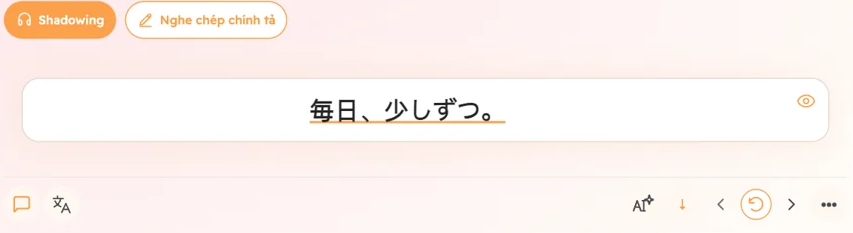
\includegraphics[width=8.4cm]{figures/ui-components/shadowing-controls.png}
  \end{minipage}\hspace{.4cm}
  \begin{minipage}[c]{5.7cm}
    \centering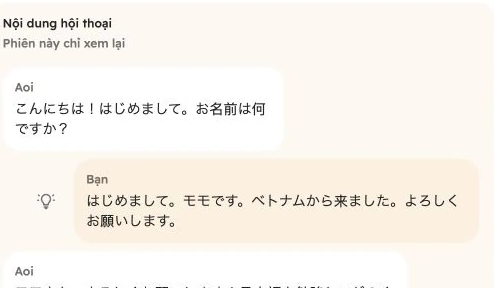
\includegraphics[width=5.7cm]{figures/ui-components/conversation-bubbles.png}
  \end{minipage}
}{Phụ đề và thanh điều khiển shadowing; các lượt hội thoại}{fig:ui-learning-interactions}

\Needspace{8cm}
\noindent\textbf{Phản hồi và hỗ trợ thao tác.}
Giao diện hiển thị trạng thái tải, xử lý và lỗi; các thao tác nộp bài được kiểm soát để tránh gửi lặp. Trong luyện viết, phần gốc và phần sửa được phân biệt bằng màu, nhãn và gạch ngang; vùng giải thích trình bày lý do chỉnh sửa để người học đối chiếu (Hình~\ref{fig:ui-writing-feedback}). Bản nháp trên web được lưu khi người học tạm dừng nhập. Bài đọc chỉ cho nộp khi đủ câu trả lời; cửa sổ viết tay dành sẵn vị trí cho năm gợi ý để hạn chế dịch chuyển bố cục.
\uicomponentfigure{
  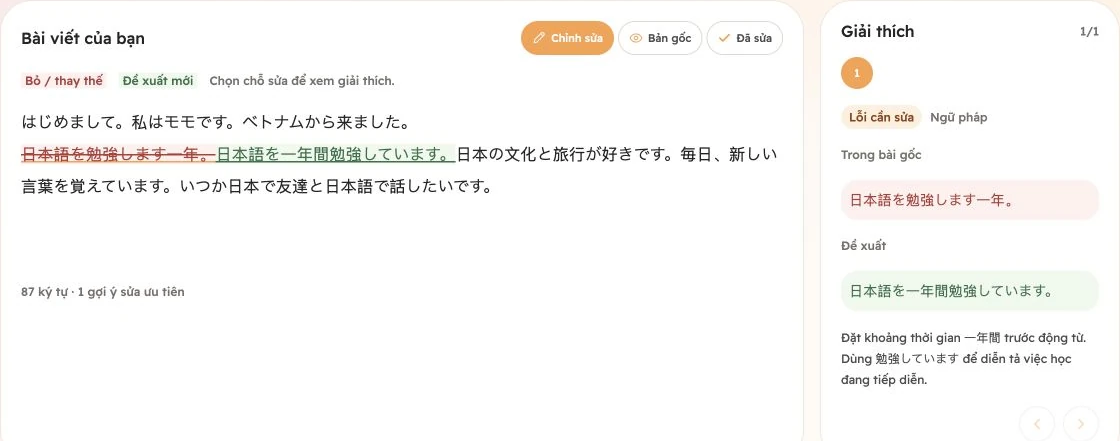
\includegraphics[width=13cm]{figures/ui-components/writing-feedback.png}
}{Thành phần hiển thị phần sửa bài viết và giải thích tương ứng}{fig:ui-writing-feedback}

\Needspace{8cm}
\noindent\textbf{Khả năng sử dụng trên nhiều thiết bị.}
Nội dung được sắp xếp theo chiều rộng màn hình. Trên di động, bộ chọn trình độ đánh dấu lựa chọn hiện tại và các thẻ bài học được bố trí theo lưới (Hình~\ref{fig:ui-mobile-lessons}); thanh điều hướng dưới có khoảng đệm cho vùng an toàn. Các điều khiển có nhãn, trạng thái chọn hoặc vô hiệu hóa; một số thành phần hỗ trợ nhãn truy cập và đường viền khi nhận focus.
\uicomponentfigure{
  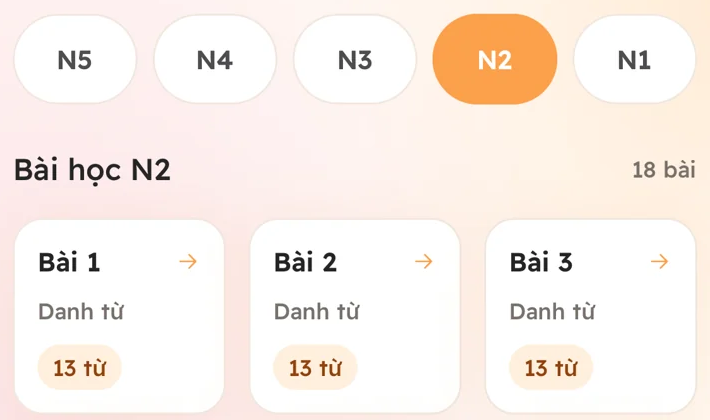
\includegraphics[width=7.5cm]{figures/ui-components/mobile-lesson-components.png}
}{Bộ chọn trình độ và các thẻ bài học trên di động}{fig:ui-mobile-lessons}
